\subsection{Evaluating Machine Energy Efficiency and Performance using Control Charts}

In this section, it is discussed on how to use the energy baseline model to identify a benchmark reporting period, monitor EE and perform PDD. Building off of \cite{oakland_statistical_2008}, the choice of the benchmark reporting period in which the model is trained on is crucial as it provides a reference to which predictions are compared to. In \cite{cas}, the authors trained their MLR on a period of one year and plotted the instantaneous and cumulative residuals. These two SPC charts allowed the authors to analyze periods of \textit{best} CAS performance indicated by the residuals fluctuating around a mean of zero. Ultimately, the baseline model was then retrained on a time period of $36$ days representing the \textit{best} performance. Here, an example of a workflow for choosing the benchmark reporting period for the paper disposal machine is given.

Using the kernel design according to the evaluation metrics in \hyperlink{table.3}{Table 3}, the model is trained on $10$ minute aggregated data from October $11^{th}$ until October $15^{th}$. In \hyperlink{figure.14}{Figure 14}, the top plot visualizes the instantaneous residuals of the in sample model fit. i.e., the difference of the predictions of the baseline model with the actual values of the benchmark reporting period. The bottom plot visualizes the cumulative residuals of the in sample fit. 

Where the SPC charts developed in this thesis differ from that in the literature and in industry is that the energy baseline model is a probabilistic model, and therefore, we have access to the uncertainty in our predictions. Where current SPC charts only take into account the point predictions and standard deviation of residuals to define UCL and LCL (as described in \hyperlink{subsection.2.3}{Section 2.3}), our proposed SPC charts utilizes the posterior distribution to define the control limits. Namely, by using the $95\%$ PI, a probabilistic approach can be used to determine the statistical significance of deviations in performance and change in EE over time. 

A red point in the top plot indicates that, at that time point $t$, the actual value was greater than $2 \sigma$ away from the mean prediction $\hat{\mu}_t$ and vice versa. Looking back at the time series plot in \hyperlink{figure.10}{Figure 10}, one can identify these outlier points. Then, in the CuSum plot, MA trend lines ($1$hr and $6$hr) are plotted to aid the identification of a benchmark reporting period. It can be seen that the slope of the residuals slightly increases until about the end of the day on October $12^{th}$, then is constant, and finally shows a slight decrease. However, in both charts, the mean of the process fluctuates around the zero bound, and thus the justification as using these four days for the benchmark reporting period is justified.

\begin{figure}[h]
\centering
\graphicspath{ {./images/} }
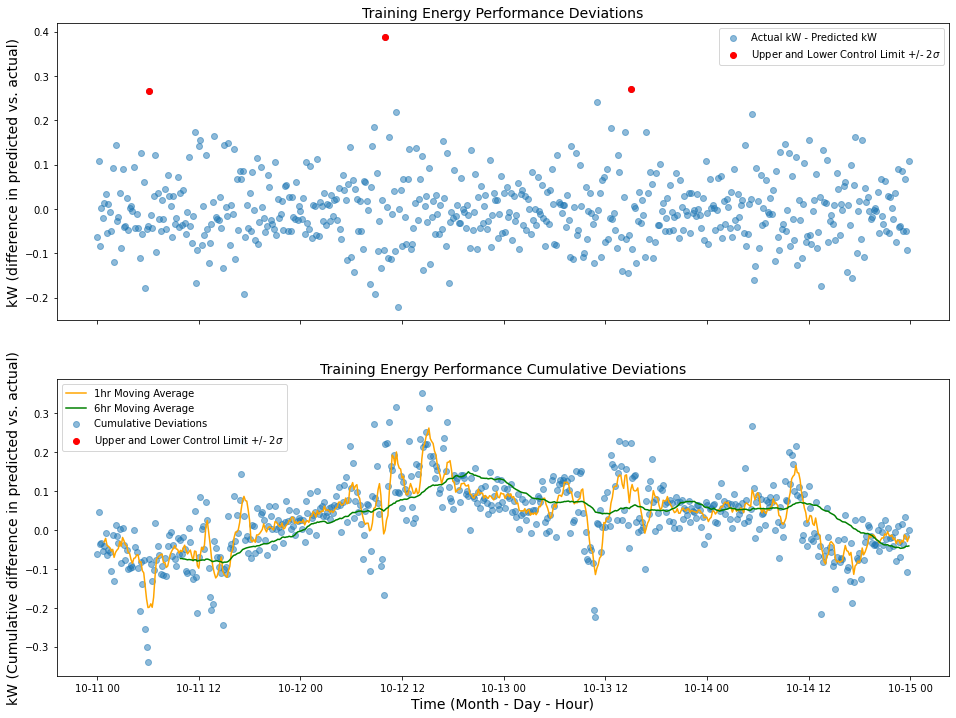
\includegraphics[scale=0.49]{images/entsorgung_baseline_SPC.png}
\caption{Entire time series for the paper disposal machine.}
\end{figure}



\subsection{Mock Model Deployment}

Docker + GitHub Actions

\subsection{Inspection of Learned Hyperparameters}

\subsection{Assumptions and Limitations of Models}

Mainly to do with the baseline reporting period. GP model complexity